\documentclass[12pt]{article}
\usepackage{amsmath,amssymb,amsthm,bm}
\usepackage{graphicx}
\usepackage{geometry}
\geometry{margin=1in}
\usepackage{tikz}
\usetikzlibrary{automata,arrows}
\usepackage{tikz}
\usetikzlibrary{arrows.meta, positioning}
\usepackage{array}
\title{Markov Chain}
\author{Thomas Huang}

\begin{document}
\maketitle
\title{}
\section*{Discrete-Time Markov Chains}

\subsection*{Overview}
We observe the state of a system at discrete times $n = 0, 1, 2, 3, \ldots$. Let $X_n$ be the state of the system at time $n$. Therefore, $\{ X_n \}$ is a discrete-time stochastic process. Two extreme cases are:
\begin{itemize}
\item $\{ X_n \}$ are i.i.d. random variables.
\item $X_n$ depends on all past states $X_{n-1}, X_{n-2}, \ldots, X_0$.
\end{itemize}

\subsection*{Markov Property}
The Markov property states that given the present state $X_n$, the future is conditionally independent of the past. Formally,
\[
P(X_{n+1} = j \mid X_n = i_n, X_{n-1} = i_{n-1}, \ldots, X_0 = i_0 )
= P(X_{n+1} = j \mid X_n = i_n).
\]
Thus, the past can only affect the future through the present state.

\subsection*{Definition of a Discrete-Time Markov Chain (DTMC)}
A stochastic process $\{X_n, n \ge 0\}$ taking values in a discrete state space $S$ is called a DTMC if:
\begin{enumerate}
\item $X_n \in S$ for all $n \ge 0$, with $S$ discrete.
\item $P(X_{n+1} = j \mid X_n = i_n, X_{n-1} = i_{n-1}, \ldots, X_0 = i_0 ) = P(X_{n+1} = j \mid X_n = i_n)$ (Markov Property)
\end{enumerate}

If the one-step transition probability does not depend on time $n$, i.e.,
\[
P_{ij}(n) = P(X_{n+1} = j \mid X_n = i) = P(X_1=j|X_0=i)= P_{ij},
\]
we call the Markov chain \emph{time-homogeneous}. In that case, $P = [P_{ij}]$ is the transition probability matrix of going from state \(i\) to \(j\), with 
\begin{itemize}
    \item $ 0\le P_{ij} \le 1$ for all $P_{ij}$
    \item $\sum_{j\in S} P_{ij} = 1$ for each $i$. (All row-sum = $1$)
\end{itemize}
Such matrix is called stochastic matrix.

\subsection*{Initial Distribution}
A DTMC is characterized by:
\begin{itemize}
\item The transition probability matrix $P$.
\item The initial distribution $\bm{a} = [a_1, a_2, \ldots, a_m]$, where $a_j = P(X_0 = j)$. 
\end{itemize}
Hence, jointly they specify the distribution of the entire chain.

\subsection*{Characterization}
$[P]$ is not sufficient to characterize a DTMC because $P_{ij}$ is not finite dimension joint distribution.
\begin{align*}
    P(X_1=5,X_0=1)&=P(X_1=5 | X_0=1)P(X_0=1)\\
    &= P_{15}P(X_0=1)\\
    &= P_{15}a_1
\end{align*}
A DTMC is uniquely characterize by [P] and its initial distribution $\textbf{a} = [a_1,a_2,...,a_j,...,a_m]$ where $a_j = P(X_0=j)$
\subsection*{Examples}

\noindent\textbf{Example 1: A Two-State Machine}\\
A machine can be in one of two states: ``up'' or ``down''. If it is up on day $n$, it remains up on day $n+1$ with probability $P_u$, otherwise it goes down with probability $1 - P_u$. If it is down on day $n$, it stays down on day $n+1$ with probability $P_d$, otherwise it goes up with probability $1 - P_d$. Denote $X_n$ as the state of the machine on day $n$ (``up'' or ``down''). \\\\
Let $X_n$ = state of the machine on day $n$.\\
This is a Markov chain with state space $S = \{\text{up}, \text{down}\}$ and transition probabilities:
\begin{align*}
    P(X_{n+1} = \text{up} \mid X_{n} &= \text{up}) = P_u \\
    P(X_{n+1} = \text{down} \mid X_{n} &= \text{up}) = 1 - P_u\\
    P(X_{n+1} = \text{up} \mid X_{n} &= \text{down}) = 1 - P_d\\
    P(X_{n+1} = \text{down} \mid X_{n} &= \text{down}) = P_d.
\end{align*}
Then the transition probability matrix $[P]$ is 
\[
[P] = 
\begin{array}{c|cc}
 & \text{to up} & \text{to down}\\\hline
\text{from up} & P_u & 1 - P_u \\
\text{from down} & 1 - P_d & P_d \\
\end{array}
\]
$\textbf{Transition Diagram}$\\
    \begin{center}
        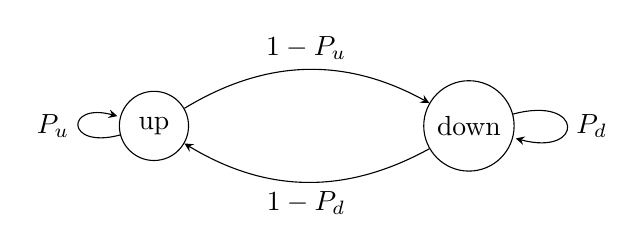
\begin{tikzpicture}[
            ->,
            >=stealth,
            node distance=4cm,
            auto
        ]
        
        % Define states
        \node[state] (up) {up};
        \node[state] (down) [right of=up] {down};
        
        % Draw transitions
        \draw (up) edge[loop left] node{$P_u$} (up);
        \draw (down) edge[loop right] node{$P_d$} (down);
        \draw (up) edge[bend left] node{$1-P_u$} (down);
        \draw (down) edge[bend left] node{$1-P_d$} (up);
        \end{tikzpicture}
    \end{center}
\begin{itemize}
\item nodes $\Rightarrow$ states (each node represents a state)
\item arcs $\Rightarrow$ transition
\end{itemize}

\noindent\textbf{Example 2: Two Independent Machines}\\
Consider two identical machines operating independently. Each machine transitions between ``up'' and ``down'' states as above. \\\\
Let $X_n$ = number of machines that are ``up'' at time $n$. \\
Then $S = \{0,1,2\}$. \\\\
For each machine:
\begin{align*}
    up \Rightarrow up \text{ with prob. } P_u\\
    down \Rightarrow down \text{ with prob. } P_d
\end{align*}
The transition probabilities can be computed based on the independence of the individual machines.
\begin{align*}
    P(X_{n+1} = 0 \mid X_{n} = 0) = P(\text{Both $M_{1,2}$ down} | \text{Both $M_{1,2}$ down}) &= P_d^2 \\
    P(X_{n+1} = 1 \mid X_{n} = 0) = P(\text{Either $M_{1,2}$ up} | \text{Both $M_{1,2}$ down})&= 2P_d(1-P_d)\\
    P(X_{n+1} = 0 \mid X_{n} = 1) = P(\text{Both $M_{1,2}$ down} | \text{Either $M_{1,2}$ up})&= P_d(1-P_u) \\
    P(X_{n+1} = 1 \mid X_{n} = 1) = P(\text{Either $M_{1,2}$ up} | \text{Either $M_{1,2}$ up}) &= P_uP_d + (1-P_u)(1-P_d)\\
    P(X_{n+1} = 2 \mid X_{n} = 0) = P(\text{Both $M_{1,2}$ up} | \text{Both $M_{1,2}$ down}) &= (1-P_d)^2\\
    P(X_{n+1} = 0 \mid X_{n} = 2) = P(\text{Both $M_{1,2}$ down} | \text{Both $M_{1,2}$ up})&= (1-P_u)^2\\
    P(X_{n+1} = 2 \mid X_{n} = 1) = P(\text{Both $M_{1,2}$ up} | \text{Either $M_{1,2}$ up})&=  P_u(1-P_d)\\
    P(X_{n+1} = 1 \mid X_{n} = 2) = P(\text{Either $M_{1,2}$ up} | \text{Both $M_{1,2}$ up)} &= 2P_u(1-P_u)\\
    P(X_{n+1} = 2 \mid X_{n} = 2) = P(\text{Both $M_{1,2}$ up} | \text{Both $M_{1,2}$ up}) &= P_u^2
\end{align*}
Then the transition probability matrix $[P]$ is 
\[
[P] = 
\begin{array}{c|ccc|ccc}
 & \text{to 0 up} & \text{to 1 up}  & \text{to 2 up} \\\hline
\text{from 0 up} & P_d^2 & 2P_d(1-P_d) & (1-P_d)^2 \\
\text{from 1 up} & P_d(1-P_u) & P_uP_d + (1-P_u)(1-P_d)& P_u(1-P_d)\\
\text{from 2 up} & (1-P_u)^2 & 2P_u(1-P_u) &P_u^2 \\
\end{array}
\]
$\textbf{Transition Diagram}$\\
\begin{center}
    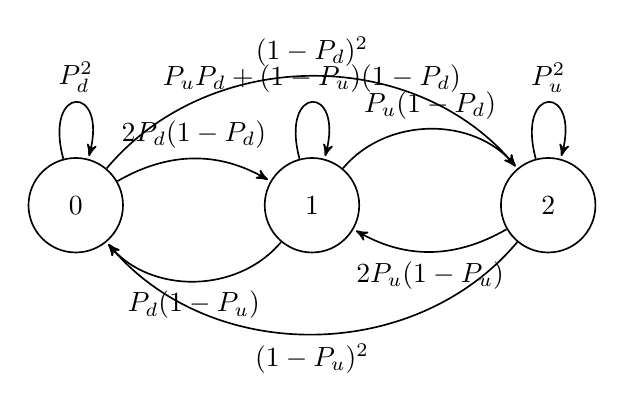
\begin{tikzpicture}[
    ->, >=stealth', shorten >=1pt, auto, node distance=3cm,
    semithick, every state/.style={circle, draw, minimum size=1.2cm}]
    
    % Define states
    \node[state] (S0) {0};
    \node[state] (S1) [right of=S0] {1};
    \node[state] (S2) [right of=S1] {2};

    % Draw transitions
    \path (S0) edge[loop above] node {$P_d^2$} (S0)
               edge[bend left] node[above] {$2P_d(1-P_d)$} (S1)
               edge[bend left=50] node[above] {$(1-P_d)^2$} (S2)
          (S1) edge[bend left=50] node[below] {$P_d(1-P_u)$} (S0)
               edge[loop above] node {$P_uP_d + (1-P_u)(1-P_d)$} (S1)
               edge[bend left=50] node[above] {$P_u(1-P_d)$} (S2)
          (S2) edge[bend left=50] node[below] {$(1-P_u)^2$} (S0)
               edge[bend left] node[below] {$2P_u(1-P_u)$} (S1)
               edge[loop above] node {$P_u^2$} (S2);

\end{tikzpicture}
\end{center}
\newpage
\noindent\textbf{Example 3: Brand Switching}\\
A customer chooses one of three brands $A, B, C$ of beer every day, and the choice on day $n+1$ depends only on the brand chosen on day $n$. State space is $S = \{A, B, C\}$. A typical transition probability matrix might be:
\[
P = \begin{pmatrix}
0.1 & 0.2 & 0.7 \\
0.2 & 0.4 & 0.4 \\
0.1 & 0.3 & 0.6
\end{pmatrix}.
\]
The entry in row $i$, column $j$ represents $P(X_{n+1}=j \mid X_n=i)$.
\\\\
$\textbf{Transition Diagram}$\\
\begin{center}
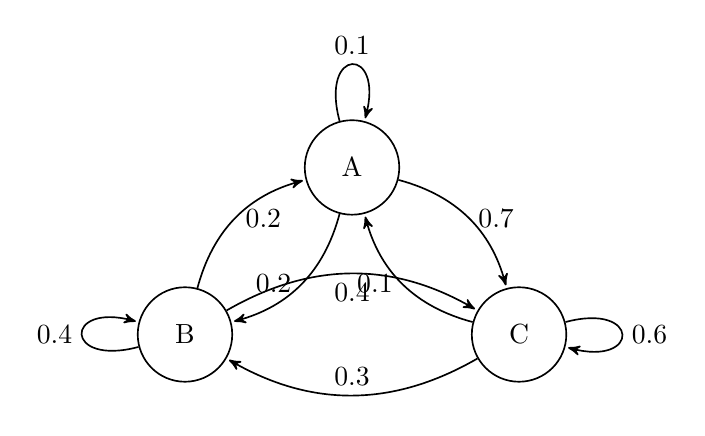
\begin{tikzpicture}[
    ->, >=stealth', shorten >=1pt, auto, node distance=3cm,
    semithick, every state/.style={circle, draw, minimum size=1.2cm}]
    
    % Define states
    \node[state] (A) {A};
    \node[state] (B) [below left of=A] {B};
    \node[state] (C) [below right of=A] {C};

    % Draw transitions
    \path (A) edge[loop above] node {$0.1$} (A)
               edge[bend left] node[left] {$0.2$} (B)
               edge[bend left] node[right] {$0.7$} (C)
          (B) edge[bend left] node[right] {$0.2$} (A)
               edge[loop left] node {$0.4$} (B)
               edge[bend left] node[below] {$0.4$} (C)
          (C) edge[bend left] node[left] {$0.1$} (A)
               edge[bend left] node[above] {$0.3$} (B)
               edge[loop right] node {$0.6$} (C);
\end{tikzpicture}
    \end{center}

\noindent\textbf{Example 4: Gambler's Ruin}\\
Person $A$ and $B$ share a total of \$N. Each bet \$1 on the flip of a coin. If the coin is heads (probability $p$), $A$ wins \$1 from $B$; otherwise $A$ loses \$1 to $B$. Let $X_n$ be the amount of money $A$ has after the $n$-th bet. Then $X_n$ takes values in $\{0,1,\ldots,N\}$, and we have a Markov chain with absorbing states $0$ and $N$ (since once $A$ has $0$ or $N$, the game ends).
\begin{center}
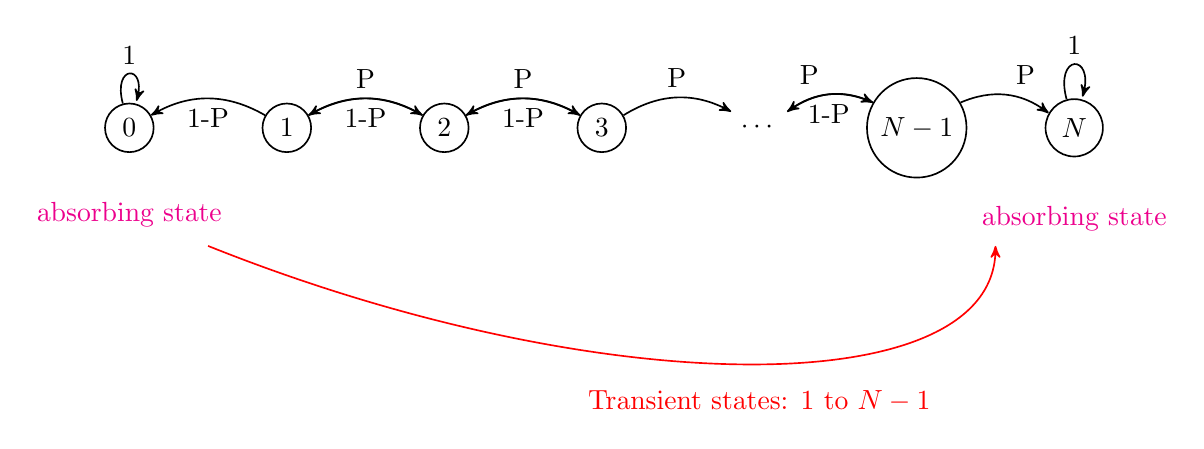
\begin{tikzpicture}[->, >=stealth', auto, node distance=2cm, semithick]

% Define nodes
\node[circle, draw] (0) at (0, 0) {0};
\node[circle, draw] (1) at (2, 0) {1};
\node[circle, draw] (2) at (4, 0) {2};
\node[circle, draw] (3) at (6, 0) {3};
\node[draw=none] (dots) at (8, 0) {$\cdots$};
\node[circle, draw] (n-1) at (10, 0) {$N-1$};
\node[circle, draw] (n) at (12, 0) {$N$};

% Absorbing state labels
\node[below=0.5cm of 0] {\textcolor{magenta}{absorbing state}};
\node[below=0.5cm of n] {\textcolor{magenta}{absorbing state}};

% Transient label
\draw[red] (1,-1.5) .. controls (6,-3.5) and (11,-3.5) .. (11,-1.5);
\node[below=3cm of dots] {\textcolor{red}{Transient states: $1$ to $N-1$}};

% Draw edges
\path 
    % Self-loops for absorbing states
    (0) edge[loop above] node {1} (0)
    (n) edge[loop above] node {1} (n)
    
    % Transitions between transient states
    (1) edge[bend left] node {P} (2)
        edge[bend right] node[below] {1-P} (0)
    (2) edge[bend left] node {P} (3)
        edge[bend right] node[below] {1-P} (1)
    (3) edge[bend left] node {P} (dots)
        edge[bend right] node[below] {1-P} (2)
    (dots) edge[bend left] node {P} (n-1)
    (n-1) edge[bend left] node {P} (n)
           edge[bend right] node[below] {1-P} (dots);

\end{tikzpicture}

\end{center}
\newpage
\subsection*{Transient Behavior(Marginal Distribution)}

The $n$-step transition probability is defined by
\[
P_{ij}^{(n)} = P(X_n = j \mid X_0 = i).
\]
The Chapman-Kolmogorov equation states:
\[
P_{ij}^{(n)} = \sum_{r \in S} P_{i r}^{(k)} \, P_{r j}^{(n-k)}, \quad 0 \le k \le n.
\]
For a time-homogeneous DTMC,
\[
P^{(n)} = P^n,
\]
where $P^{(n)} = [P_{ij}^{(n)}]$ is the $n$-step transition matrix. The distribution of $X_n$ is then
\[
P(X_n = j) = \sum_{i \in S} P(X_n = j \,\mid\, X_0 = i)\,P(X_0 = i) = \sum_{i \in S} P_{ij}^{(n)}\, a_i,
\]
or in vector form,
\[
\bm{a}^{(n)} = \bm{a}\,P^{(n)} = \bm{a}\,P^n.
\]

\subsubsection*{Example}
Let $\{X_n\}$ be a DTMC. Let $S=\{1,2,3,4\}$ and 
\[
   [P] =  \begin{bmatrix}
0.1 & 0.2 & 0.3 & 0.4\\
0.2 & 0.2 & 0.3 & 0.3 \\
0.5 & 0 & 0.5 & 0\\
0.6 & 0.2 & 0.1 & 0.1
\end{bmatrix}
\]
and initial distribution 
\[
\textbf{a} = \begin{bmatrix}
0.25 \\
0.25 \\
0.25 \\
0.25 
\end{bmatrix}
\]
Find $P(X_3=4,X_2=1,X_1=3,X_0=1)$, $P(X_3=4,X_2=1,X_1=3)$, $a^{(n)}$\\\\
(1)
\begin{align*}
    P(X_{3}=4,\,X_{2}=1,\,X_{1}=3,\,X_{0}=1)
    &= P(X_{3}=4 \mid X_{2}=1,\,X_{1}=3,\,X_{0}=1)\\
     &  P(X_{2}=1 \mid X_{1}=3,\,X_{0}=1)\\
     &  P(X_{1}=3 \mid X_{0}=1)  P(X_{0}=1)\\
    &=P(X_{3}=4 \mid X_{2}=1)P(X_{2}=1 \mid X_{1}=3)\\
     &  P(X_{1}=3 \mid X_{0}=1)  P(X_{0}=1)\\
    &= p_{14}\,p_{13}\,p_{13}\,a_{1}\\
    &= 0.4 \times 0.5 \times 0.3 \times 0.25\\
    &= 0.015
\end{align*}
(2)
\begin{align*}
P(X_{3}=4,X_{2}=1, X_{1}=3)
&= \sum_{i=1}^{4} P\bigl(X_{3}=4,\,X_{2}=1,\,X_{1}=3,\,X_{0}=i\bigr)\\
&= \sum_{i=1}^{4} (P(X_{3}=4 \mid X_{2}=1,\,X_{1}=3,\,X_{0}=i)\\
     &  P(X_{2}=1 \mid X_{1}=3,\,X_{0}=i)\\
     &  P(X_{1}=3 \mid X_{0}=i)  P(X_{0}=i))\\
&= P(X_{3}=4 \mid X_{2}=1,\,X_{1}=3,\,X_{0}=i)\\
     &  P(X_{2}=1 \mid X_{1}=3,\,X_{0}=i)\\
     &   \sum_{i=1}^{4} (P(X_{1}=3 \mid X_{0}=i)  P(X_{0}=i))\\
&= p_{31}\,p_{14}\,\Bigl(\sum_{i=1}^{4} a_{i}\,p_{i3}\Bigr)\\
&= 0.5 \times 0.4 \times \Bigl[\,0.25 \times (0.3 + 0.3 + 0.5 + 0.1)\Bigr]\\
&= 0.06
\end{align*}
(3)
\begin{align*}
a^{(4)} &= p^{(4)}\,a^{(0)} \;=\; p^4\,a,\\
a^{(1)} 
&= \begin{pmatrix}
0.341\\
0.135\\
0.325\\
0.198
\end{pmatrix}
\end{align*}
\section*{Limiting Behavior of a DTMC}

\[
\lim_{n \to \infty} a_{j}^{(n)} = \lim_{n \to \infty} P(X_{n} = j)
\]
\[
a^{(n)} = P^n \, a
\]
\[
\lim_{n \to \infty} a^{(n)} = \lim_{n \to \infty}  \, P^n \, a
\]
\[
\lim_{n \to \infty} a^{(n)} = a\lim_{n \to \infty} \, P^n
\]

\subsection*{Example: Brand Switching}

A customer buys beer every day among 3 different brands \(A, B, C\). The choice on day \(n+1\) depends only on the choice on day \(n\). Let \(X_{n}\) be the brand choice on day \(n\). Suppose
\[
X_{n} \in \{A, B, C\}, \quad
P = \begin{bmatrix}
0.1 & 0.2 & 0.7 \\
0.2 & 0.4 & 0.4 \\
0.1 & 0.3 & 0.6
\end{bmatrix}
\]
Suppose the initial distribution is
\[
a = \bigl[\,0.2 \quad 0.3 \quad 0.5\bigr].
\]
The question is: What is the long-run market share of a particular brand?

\[
a^{(1)} =
\begin{bmatrix}
0.13 \\
0.31 \\
0.56
\end{bmatrix}
\quad
\text{As } n \text{ gets larger,}
\quad
P^n =
\begin{bmatrix}
0.132 & 0.319 & 0.549 \\
0.132 & 0.319 & 0.549 \\
0.132 & 0.319 & 0.549
\end{bmatrix}.
\]
Hence, the limit distribution exists (the rows become identical). Therefore, no matter what \(a\) is,
\[
\lim_{n \to \infty} a^{(n)} =
\bigl[\,0.132 \quad 0.319 \quad 0.549\bigr].
\]
(The limiting distribution is unaffected by the choice of \(a\).)\\\\
What if \[
[P] = \begin{bmatrix}
    0 & 1& 0 \\
    0.5 & 0 &  0.5\\
    0 & 1 & 0
\end{bmatrix}
\]
When $n$ gets larger then
\[
P^{(2k)} =
\begin{bmatrix}
    0.5 & 0& 0.5 \\
    0 & 1 &  0\\
    0.5 & 0 & 0.5
\end{bmatrix}
\quad
P^{(2k+1)} =
\begin{bmatrix}
    0 & 1 &  0 \\
    0.5 & 0 & 0.5\\
    0 & 1 &  0
\end{bmatrix}
\]
Their corresponded limiting distribution is
\begin{align*}
    a^{(2k)} &= a \cdot P^{(2k)}\\
    &= \begin{bmatrix}
        0.35\\
        0.3\\
        0.35
    \end{bmatrix}
\end{align*}
\begin{align*}
    a^{(2k+1)} &= a \cdot P^{(2k+1)}\\
    &= \begin{bmatrix}
        0.15\\
        0.7\\
        0.15
    \end{bmatrix}
\end{align*}
limiting distribution does not exist also the distribution depends on the choices of $\textbf{a}$.\\\\
So, under what condition does limiting distribution exist?\\
- periodicity \\\\
If it exists limiting distribution, when is it dependent of the choice of the initial distribution $\textbf{a}$?\\
- irreducibility

\subsection*{Section 6.2.1 Classification of States (Irreducibility, periodicity)}

\subsubsection*{Accessible} A state \(j\) is said to be \emph{accessible} from state \(i\) if there exists an \(n\) such that
\[
P_{ij}^{(n)} = P(X_{n} = j \mid X_{0} = i) > 0.
\]
Write \(i \to j\) if \(i\) is accessible to \(j\). Clearly \(i \to i\) for any state \(i\).

\subsubsection*{Communicate} A state \(i\) is said to \emph{communicate} with \(j\) (written \(i \leftrightarrow j\)) if \(i \to j\) and \(j \to i\).

\subsubsection*{Theorem} If \(i \leftrightarrow j\) and \(j \leftrightarrow k\), then \(i \leftrightarrow k\).

\subsubsection*{Communicating class} A set \(C \subseteq S\) is said to be a \emph{communicating class} if for any \(i, j \in C\), \(i \leftrightarrow j\) holds.

\subsubsection*{Closeure} A communicating class \(C\) is said to be \emph{closed} if whenever \(i \in C\) and \(i \to j\), then \(j \in C\). Otherwise, \(C\) is \emph{open}.

If \(X_n \in C\) for some \(n\), then \(X_m \in C\) for all \(m \ge n\).

\subsubsection*{Definition} A DTMC is said to be \emph{irreducible} if all its states belong to a single closed communicating class. Otherwise it is \emph{reducible}.
\newpage
\subsubsection*{Example}
Example 1: 
\[
S = \{1, 2\}
\]

\[
P = 
\begin{pmatrix}
0.2 & 0.8 \\
0.3 & 0.7
\end{pmatrix}
\]
\begin{center}
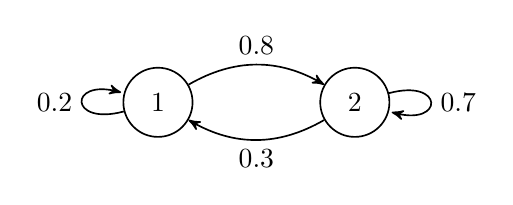
\begin{tikzpicture}[->, >=stealth', auto, node distance=2.5cm, semithick]
    \node[state] (1) {1};
    \node[state] (2) [right of=1] {2};

    \path
        (1) edge [loop left] node {0.2} (1)
            edge [bend left] node {0.8} (2)
        (2) edge [loop right] node {0.7} (2)
            edge [bend left] node {0.3} (1);
\end{tikzpicture}
\end{center}
Relationship:\\
\begin{itemize}
    \item $1 \xleftarrow{}2$
    \item $1 \xrightarrow{}2$
        \begin{itemize}
            \item Since $1 \xleftarrow{}2$ and $1 \xrightarrow{}2$ So, $1 \leftrightarrow2$
        \end{itemize}
    \item $1 \leftrightarrow 1$
    \item $2 \leftrightarrow 2$
\end{itemize}
\textbf{So this chain is irreducible since it consists only one communication class}
\\\\
Example 2:
\[
P = \begin{pmatrix}
1 & 0 \\
0.3 & 0.7
\end{pmatrix}
\quad
S = \{1,2\}
\]
\begin{center}
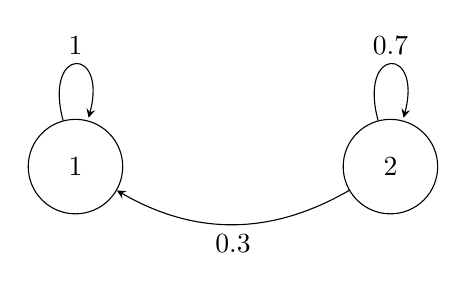
\begin{tikzpicture}[->, >=stealth, auto, node distance=3cm,
  state/.style={circle, draw, minimum size=1.2cm}]
  \node[state] (1) at (0,0) {1};
  \node[state] (2) at (4,0) {2};

  % transitions
  \path (1) edge[loop above] node{$1$} (1);
  \path (2) edge[loop above] node{$0.7$} (2);
  \path (2) edge[bend left] node{$0.3$} (1);
\end{tikzpicture}
\end{center}
Relationship:\\
\begin{itemize}
    \item $1 \leftrightarrow1$
        \begin{itemize}
            \item {1} is a closed communication class
        \end{itemize}
    \item $2 \xrightarrow{}1$ 
    \item $2 \leftrightarrow 2$
        \begin{itemize}
            \item {2} is a opened communication class
        \end{itemize}
\end{itemize}
\textbf{So this chain is reducible since it consists two communication classes}\\\\
Example 3:
\[
P = \begin{pmatrix}
1 & 0 \\
0 & 1
\end{pmatrix}
\]
\begin{center}
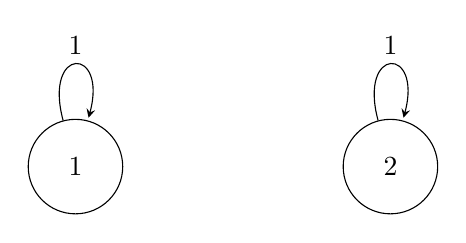
\begin{tikzpicture}[->, >=stealth, auto, node distance=3cm,
  state/.style={circle, draw, minimum size=1.2cm}]
  \node[state] (1) at (0,0) {1};
  \node[state] (2) at (4,0) {2};

  % transitions
  \path (1) edge[loop above] node{$1$} (1);
  \path (2) edge[loop above] node{$1$} (2);
\end{tikzpicture}
\end{center}
Relationship:\\
\begin{itemize}
    \item $1 \leftrightarrow1$
        \begin{itemize}
            \item {1} is a closed communication class
        \end{itemize}
    \item $2 \leftrightarrow2$
        \begin{itemize}
            \item {2} is a closed communication class
        \end{itemize}
\end{itemize}
\textbf{So this chain is reducible since it consists two communication classes}\\\\
Example 3: Random Walk on {0,1,...,N}\\
$p$ = probability of stepping right\\
$(1-p)$ = probability of stepping left

\[
\text{Random walk states: } \{0,1,\ldots,N\}, 
\quad \text{Transitions: } 
P(i \xrightarrow{} i+1)=p,\;
P(i\xrightarrow{} i-1)=1-p\,
\]
\begin{center}
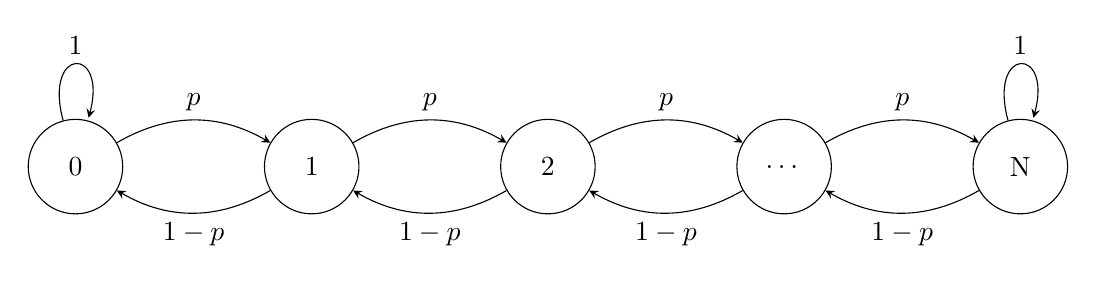
\begin{tikzpicture}[->, >=stealth, auto, node distance=2cm,
  state/.style={circle, draw, minimum size=1.2cm}]
  % States
  \node[state] (0) at (0,0)  {0};
  \node[state] (1) at (3,0)  {1};
  \node[state] (2) at (6,0)  {2};
  \node[state] (dots) at (9,0)  {$\dots$};
  \node[state] (N) at (12,0) {N};

  % Transitions for 0 and N (closed classes)
  \path (0) edge[loop above] node{1} (0);
  \path (N) edge[loop above] node{1} (N);

  % Transitions among 1, 2, ..., N-1
  \path (1) edge[bend left]  node{$p$} (2);
  \path (2) edge[bend left]  node{$1-p$} (1);

  % Indicate a chain of similar transitions
  % skipping the explicit middle ones with the "..." node
  \draw[->] (dots) to[bend left] node{$p$} (N);
  \draw[->] (2) to[bend left] node{$p$} (dots);
  \draw[->] (dots) to[bend left] node{$1-p$} (2);
  \draw[->] (N) to[bend left] node{$1-p$} (dots);
  \draw[->] (1) to[bend left] node{$1-p$} (0);
  \draw[->] (0) to[bend left] node{$p$} (1);
\end{tikzpicture}
\end{center}
% Note: {0} and {N} form closed communicating classes; {1,...,N-1} is open.
Relationship:\\
\begin{itemize}
    \item $0 \leftrightarrow 0$
        \begin{itemize}
            \item $\{0\}$ is a closed communication class
        \end{itemize}
    \item $N \leftrightarrow N$
        \begin{itemize}
            \item $\{N\}$ is a closed communication class
        \end{itemize}
    \item $0 \leftarrow 1$
    \item $N-1 \rightarrow N$
    \item $i \leftrightarrow i+1$ for $i=1,2,...,N-1$
        \begin{itemize}
            \item $\{1,2,...,N-1\}$ is a opened communication class
        \end{itemize}
\end{itemize}
\textbf{So this chain is reducible since it consists three communication classes}
\subsubsection*{Periodicity}
A state $i$ is said to be \emph{periodic} with period d if d is the largest integer such that
\[
    P^{(n)}_{ii} = P(X_n=i|X_0=i) > 0 \Rightarrow \text{ is an integer multiple of } d  
\]
If $d$ = 1, $i$ is called \emph{aperiodic}.\\\\
Ex) The set of integers $n$ for which $p_{ii}^{(n)} > 0$ is given by:
\[
\{\,0,\,3,\,7,\,9,\,11,\,\dots\} \implies \gcd=1 \text{ (aperiodic)},
\]
\[
\{\,0,\,3,\,6,\,9,\,12,\,15,\,\dots\} \implies \gcd=3 \text{ (periodic)},
\]
\[
\{\,0,\,1,\,3,\,3,\,6,\,9,\,12,\,15,\,\dots\} \implies \gcd=1 \text{ (aperiodic)}.
\]
\textbf{Theorem}: If $i \leftrightarrow j,$ then $i$ and $j$ have the same period. All states in a communicating class share the same period.
\\\\
Ex) In a chain with transition probability $p$, suppose
\[
P_{00} = 1 \;>\; 0 \quad \implies \quad d=1 \quad (\text{aperiodic}),
\]
and if $P_{nn} = 1 \;>\; 0$, then $d=1$ again (aperiodic). However, if from any state one needs $2n$ steps to return to state 1, then $d=2$ (periodic).
\\\\
Ex)
\begin{center}
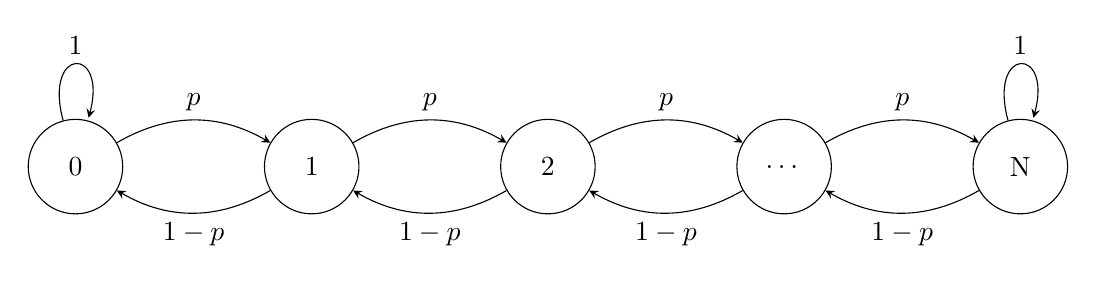
\begin{tikzpicture}[->, >=stealth, auto, node distance=2cm,
  state/.style={circle, draw, minimum size=1.2cm}]
  % States
  \node[state] (0) at (0,0)  {0};
  \node[state] (1) at (3,0)  {1};
  \node[state] (2) at (6,0)  {2};
  \node[state] (dots) at (9,0)  {$\dots$};
  \node[state] (N) at (12,0) {N};

  % Transitions for 0 and N (closed classes)
  \path (0) edge[loop above] node{1} (0);
  \path (N) edge[loop above] node{1} (N);

  % Transitions among 1, 2, ..., N-1
  \path (1) edge[bend left]  node{$p$} (2);
  \path (2) edge[bend left]  node{$1-p$} (1);

  % Indicate a chain of similar transitions
  % skipping the explicit middle ones with the "..." node
  \draw[->] (dots) to[bend left] node{$p$} (N);
  \draw[->] (2) to[bend left] node{$p$} (dots);
  \draw[->] (dots) to[bend left] node{$1-p$} (2);
  \draw[->] (N) to[bend left] node{$1-p$} (dots);
  \draw[->] (1) to[bend left] node{$1-p$} (0);
  \draw[->] (0) to[bend left] node{$p$} (1);
\end{tikzpicture}
\end{center}
\begin{itemize}
    \item For $\{0\}$ Class: $P_{00} = 1 > 0$, so $d=1$. Therefore, aperiodic.
    \item For $\{1,2,..,N-1\}$ Class: Pick a random state. For example, 1, then the steps to come back to state 1 from any state is $2n$, so $d=2$. Therefore, periodic.
    \item For $\{N\}$ Class: $P_{NN} = 1 > 0$, so $d=1$. Therefore, aperiodic.
\end{itemize}
\newpage
\section*{Recurrence and Transience}
When thinking about the long-run behaviour of Markov chains, it’s useful to classify two different types of states: \emph{recurrent} states and \emph{transient} states.

\begin{table}[h!]
\centering
\renewcommand{\arraystretch}{1.5}
\begin{tabular}{|m{6cm}|m{6cm}|}
\hline
\textbf{Recurrent states} & \textbf{Transient states} \\ 
\hline
If we ever visit \(i\), then we keep returning to \(i\) again and again & We might visit \(i\) a few times, but eventually we leave \(i\) and never come back \\ 
\hline
Starting from \(i\), the expected number of visits to \(i\) is infinite & Starting from \(i\), the expected number of visits to \(i\) is finite \\ 
\hline
Starting from \(i\), the number of visits to \(i\) is certain to be infinite & Starting from \(i\), the number of visits to \(i\) is certain to be finite \\ 
\hline
The return probability \(f_i\) equals 1 & The return probability \(f_i\) is strictly less than 1 \\ 
\hline
\end{tabular}
\caption{Comparison of recurrent and transient states in Markov chains.}
\end{table}
\subsection*{Definition of First Passage Time}
Fix a state $i$. Define the first passage time:
\[ T_i = \min\{n > 0: X_n = i\} \]
$T_i$ is an integer-valued random variable.

Let $f_i = P(T_i < \infty | X_0 = i)$ be the probability that state $i$ will be revisited by the MC.

\subsection*{Recurrent and Transient States}
\subsection*{Definition}
A state $i$ is called:
\begin{itemize}
    \item recurrent if $f_i = 1$
    \item transient if $f_i < 1$
\end{itemize}
\newpage
\subsection*{Intuitive Interpretation}
Let $N =$ Total times state $i$ is visited by the MC
\begin{itemize}
    \item For recurrent $i$: $E[N|X_0 = i] = \infty$
    \begin{center}
        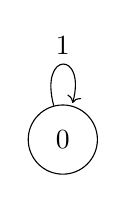
\begin{tikzpicture}
            \node[state] (0) at (0,0)  {0};
            \path (0) edge[loop above] node{1} (0);
        \end{tikzpicture}
    \end{center}
    \item For transient $i$: $E[N|X_0 = i] = \frac{1}{1-f_i}$
    \begin{center}
        \begin{tikzpicture}
            \node[state] (0) at (0,0)  {0};
            \path (0) edge[loop above] node{$f_i$} (0);
            \path (0) edge[bend left]  node{$1-f_i$} (1);
        \end{tikzpicture}
    \end{center}
    \item $P(N = k|X_0 = i) = f_i^{k-1}(1-f_i)$
\end{itemize}

\subsection*{Necessary and Sufficient Conditions}
\textbf{Theorem: }
A state $i$ is:
\begin{itemize}
    \item recurrent if and only if $\sum_{n=0}^{\infty} P_{ii}^{(n)} = \infty$
    \item transient if and only if $\sum_{n=0}^{\infty} P_{ii}^{(n)} < \infty$
\end{itemize}

\begin{proof}[Proof Sketch]
Let $Y_n = \begin{cases} 1 & \text{if } X_n = i \\ 0 & \text{if } X_n \neq i \end{cases}$

Then:
\[ E[N|X_0 = i] = E[\sum_{n=0}^{\infty} Y_n|X_0 = i] = \sum_{n=0}^{\infty} E[Y_n|X_0 = i] = \sum_{n=0}^{\infty} P_{ii}^{(n)} \]
\end{proof}

\subsection*{Class Properties}
\begin{enumerate}
    \item If state $i$ is recurrent and $i \leftrightarrow j$, then $j$ is also recurrent
    \item If state $i$ is transient and $i \leftrightarrow j$, then $j$ is also transient
    \item An irreducible DTMC is recurrent/transient if all of its states are recurrent/transient
\end{enumerate}

\subsection*{Finite Communicating Classes}
\begin{enumerate}
    \item Let $C$ be a finite closed communicating class. All states in $C$ are recurrent.
    \item Let $C$ be a finite open communicating class. All states in $C$ are transient.
    \item If $S$ is finite, all communicating classes are finite (either open or closed).
\end{enumerate}
\subsection*{Example}
(1) Given a transition matrix:
\begin{center}
    $[P] = 
    \begin{bmatrix}
        0&0&\frac{1}{2}&\frac{1}{2}\\
        1&0&0&0\\
        0&1&0&0\\
        0&1&0&0
    \end{bmatrix}$
\end{center}
We can create a transition diagram:
\begin{center}
    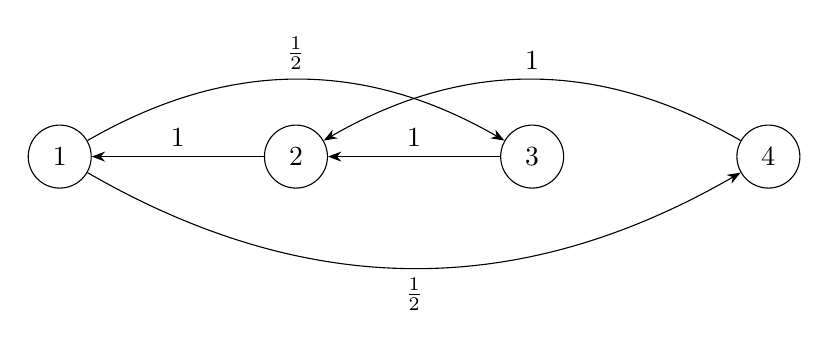
\begin{tikzpicture}[
    node distance=3cm,
    state/.style={circle,draw,minimum size=0.8cm}
    ]
    % Nodes
    \node[state] (1) {1};
    \node[state] (2) [right of=1] {2};
    \node[state] (3) [right of=2] {3};
    \node[state] (4) [right of=3] {4};
    
    % Straight arrows with probability 1
    \draw[-{Stealth[]}] (3) -- node[above] {1} (2);
    \draw[-{Stealth[]}] (2) -- node[above] {1} (1);
    
    % Upper curved arrow from 1 to 3 with probability 1/2
    \draw[-{Stealth[]}] (1) to[bend left=30] node[above] {$\frac{1}{2}$} (3);
    
    % Lower curved arrow from 1 to 4 with probability 1/2
    \draw[-{Stealth[]}] (1) to[bend right=30] node[below] {$\frac{1}{2}$} (4);
    
    % Arrow from 4 to 2 with probability 1
    \draw[-{Stealth[]}] (4) to[bend right=30] node[above] {1} (2);
\end{tikzpicture}
\end{center}
\begin{itemize}
    \item $\{1,2,3,4\}$ forms a single communicating class
    \item The chain is irreducible 
    \item The class is closed
    \item Therefore, all states are recurrent
\end{itemize}
\newpage
(2) Given a transition matrix:
\begin{center}
    $[P] = 
    \begin{bmatrix}
        \frac{1}{2}&\frac{1}{2}&0&0&0\\
        \frac{1}{2}&\frac{1}{2}&0&0&0\\
        0&0&\frac{1}{2}&\frac{1}{2}&0\\
        \frac{1}{4}&\frac{1}{4}&0&0&\frac{1}{2}
    \end{bmatrix}$
\end{center}
We can create a transition diagram:
\begin{center}
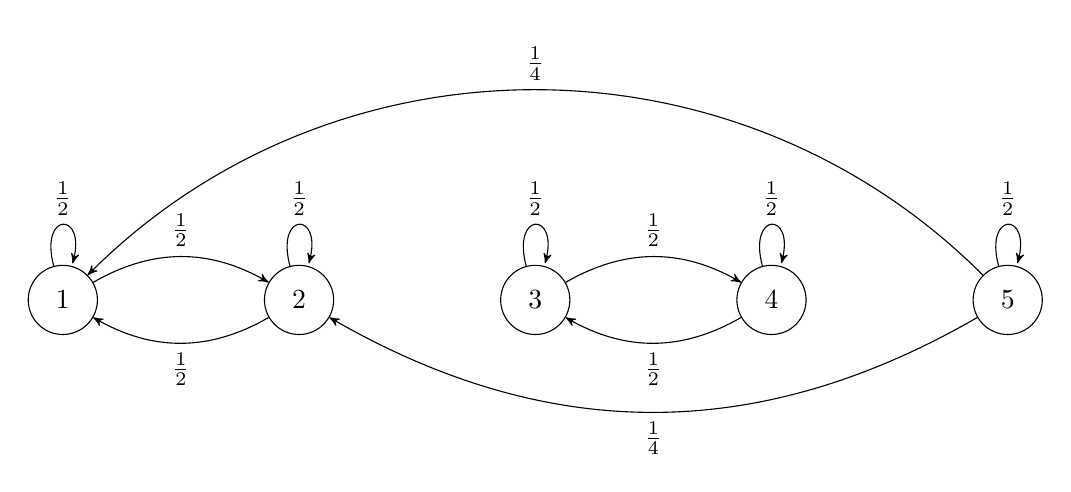
\begin{tikzpicture}[->,>=stealth',auto,node distance=3cm]
    % Define the states in a horizontal line
    \node[state] (1) {1};
    \node[state] (2) [right of=1] {2};
    \node[state] (3) [right of=2] {3};
    \node[state] (4) [right of=3] {4};
    \node[state] (5) [right of=4] {5};
    
    % Self loops
    \path (1) edge[loop above] node{$\frac{1}{2}$} (1);
    \path (2) edge[loop above] node{$\frac{1}{2}$} (2);
    \path (3) edge[loop above] node{$\frac{1}{2}$} (3);
    \path (4) edge[loop above] node{$\frac{1}{2}$} (4);
    \path (5) edge[loop above] node{$\frac{1}{2}$} (5);
    
    % Transitions between states
    \path (1) edge[bend left=30] node[above] {$\frac{1}{2}$} (2);
    \path (2) edge[bend left=30] node[below] {$\frac{1}{2}$} (1);
    
    \path (3) edge[bend left=30] node[above] {$\frac{1}{2}$} (4);
    \path (4) edge[bend left=30] node[below] {$\frac{1}{2}$} (3);
    
    \path (5) edge[bend right=45] node[above] {$\frac{1}{4}$} (1);
    \path (5) edge[bend left=30] node[below] {$\frac{1}{4}$} (2);
\end{tikzpicture}
\end{center}
\begin{itemize}
    \item $\{1,2\}$ closed recurrent communicating class
    \item $\{3,4\}$ closed recurrent communicating class
    \item $\{5\}$ open transient communicating class
\end{itemize}
\section*{Limiting Behavior of Irreducible DTMCs}

Suppose the state space \(S\) is finite.

\subsection*{Theorem 1}
For finite irreducible DTMCs, there exists a unique stationary distribution vector 
\[
    \pi = [\pi_1, \pi_2, \ldots, \pi_m]
\]
, satisfying:
\begin{itemize}
    \item  \(\pi P = \pi,\)
    \item  \(\sum_{j=1}^m \pi_j = 1,\)
    \item  Each entry of \(\pi_j > 0.\)
\end{itemize}


\subsection*{Theorem 2 (Ergodic Theorem)}
For finite irreducible aperiodic DTMCs:
\begin{itemize}
    \item The limiting probability exists:
    \[
    P_{ij}^{(n)} \to \pi_j, \quad n \to \infty.
    \]
    \item In the aperiodic case: $\pi$ is the limiting distribution.
    \item The stationary distribution satisfies:
    \begin{itemize}
        \item Long-run fraction of time spent in state \(j:\)
        \[
        E[\text{time in } j] = \pi_j.
        \]
        \item if $a = \pi$ then $\pi$ is called the steady state distribution.
    \end{itemize}
    
\end{itemize}

\subsection*{Theorem 3}
For finite irreducible periodic DTMCs:
\begin{itemize}
    \item The limiting probability \(P_{ij}^{(n)}\) does not exist.
    \item However, a stationary distribution still exists and satisfies:
    \[
    \pi P = \pi.
    \]
\end{itemize}


\section*{Examples}

\subsection*{Example 1: Brand Switching}
Consider a DTMC with three states (\(A, B, C)\), transition matrix:
\[ 
P =
    \begin{bmatrix}
        0.1 & 0.2 & 0.7 \\ 
        0.2 & 0.4 & 0.4 \\ 
        0.1 & 0.3 & 0.6
    \end{bmatrix}.
\]
Initial distribution: 
\[a^{(0)} = [a_A, a_B, a_C] = [0.2, 0.3, 0.5].\]
Transition Diagram:

\begin{center}
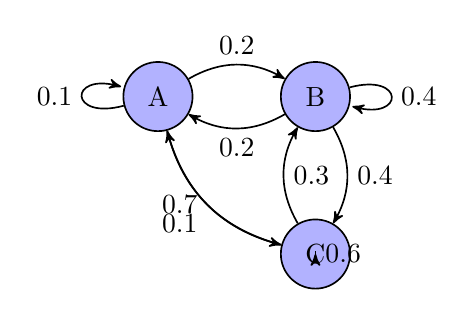
\begin{tikzpicture}[->, >=stealth', auto, semithick, node distance=2cm]
\tikzstyle{every state}=[fill=blue!30!white,draw=black,text=black]

\node[state] (A) {A};
\node[state] (B) [right of=A] {B};
\node[state] (C) [below of=B] {C};

\path 
(A) edge[bend left] node {0.2} (B)
    edge[loop left] node {0.1} (A)
    edge[bend right] node[left] {0.7} (C)
(B) edge[bend left] node {0.4} (C)
    edge[bend left] node {0.2} (A)
    edge[loop right] node {0.4} (B)
(C) edge[bend left] node[right] {0.3} (B)
    edge[bend right] node[right] {0.6} (C)
    edge[bend left] node {0.1} (A);
\end{tikzpicture}
\end{center}
Long-Run Behavior: 
As \(n \to \infty,\) the long-run market share stabilizes at:
\[
\pi = [\pi_A, \pi_B, \pi_C] = [0.132, 0.319, 0.549].
\]

\subsection*{Example 2: Periodic DTMC}
Consider the following transition matrix:
\[ 
P =
    \begin{bmatrix}
        0 & 1 \\ 
        1 & 0
    \end{bmatrix}.
\]

This chain is periodic with period \(d = 2.\)\\
Transition Diagram:

\begin{center}
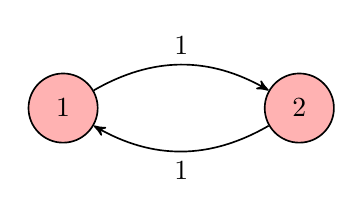
\begin{tikzpicture}[->, >=stealth', auto, semithick, node distance=3cm]
\tikzstyle{every state}=[fill=red!30!white,draw=black,text=black]

\node[state] (1) {1};
\node[state] (2) [right of=1] {2};

\path 
(1) edge[bend left] node {1} (2)
(2) edge[bend left] node {1} (1);
\end{tikzpicture}
\end{center}

In this case: The limiting distribution does not exist due to periodicity.

\subsection*{Example 3: Aperiodic DTMC}
Consider the following transition matrix:
\[ 
P =
    \begin{bmatrix}
        0.3 & 0.7 \\ 
        0.6 & 0.4
    \end{bmatrix}.
\]

This chain is irreducible and aperiodic.
Transition Diagram:

\begin{center}
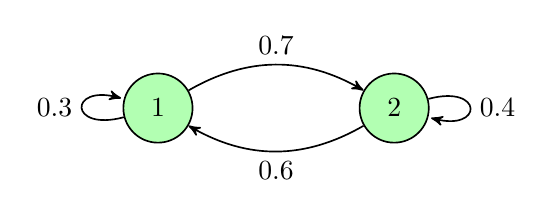
\begin{tikzpicture}[->, >=stealth', auto, semithick, node distance=3cm]
\tikzstyle{every state}=[fill=green!30!white,draw=black,text=black]

\node[state] (1) {1};
\node[state] (2) [right of=1] {2};

\path 
(1) edge[bend left] node {0.7} (2)
    edge[loop left] node {0.3} (1)
(2) edge[bend left] node {0.6} (1)
    edge[loop right] node {0.4} (2);
\end{tikzpicture}
\end{center}

In this case: The limiting distribution exists and is given by:
    \[
    \pi = [\pi_1, \pi_2] = [0.462, 0.538].
    \]
\end{document}